\chapter{Datenverarbeitung (Data Preprocessing)}

Im Folgenden wird die Datenverarbeitung, insbesondere das Data Preprocessing, in all ihren wichtigen Aspekten behandelt.
Hierbei werden die Schritte der Datenbereinigung, Datennormalisierung und Datenaugmentierung erläutert.
Diese grundlegenden Vorverarbeitungsschritte sind unverzichtbar, um hochwertige Daten zu erhalten, die für Analysen und Modellierungszwecke geeignet sind.

\section{Was sind Daten? Natur der Daten}

Eine präzise Definition von Daten ist von zentraler Bedeutung, um ein umfassendes Verständnis der Datenverarbeitung zu gewährleisten.
Daten repräsentieren Informationen oder Fakten, die aus verschiedenen Quellen und in unterschiedlichen Formen gesammelt werden.
Sie dienen als Grundlage (Ground truth) für Analysen und Modellbildung, um Muster und Erkenntnisse zu identifizieren, die zur Lösung von Problemen oder zur Gewinnung von Informationen dienen.

\section{Die Bedeutung von qualitativ hochwertigen Daten}

In der Welt der Datenanalyse und des maschinellen Lernens ist die Qualität der Daten von entscheidender Bedeutung.
Daten können fehlerhaft, inkonsistent oder unvollständig sein, da sie aus unterschiedlichen Quellen, von all-möglichen Quellen annotiert werden und in verschiedenen Formaten stammen.
Die Resultate und Ergebnisse welche die Modelle zurückgegeben, stehen in direkter Korrelation zur Qualität der genutzten Trainingsdaten\footfullcite{rahm2000data}.
Um zuverlässige und aussagekräftige Ergebnisse zu erzielen, ist es unerlässlich, die Daten zu bereinigen und sicherzustellen, dass sie für Analysen und Modellierungszwecke geeignet sind.
Dieser kritische Prozess wird als Datenbereinigung oder Data Cleaning bezeichnet.

Die Datenbereinigung beinhaltet den Prozess, fehlerhafte, inkonsistente oder unvollständige Daten aus einem Datensatz zu entfernen.
Das Hauptziel besteht darin, die Datenqualität zu verbessern und sicherzustellen, dass sie für die weiteren Schritte der Datenanalyse und des maschinellen Lernens verwendet werden können.
Eine sorgfältige Datenbereinigung ist von entscheidender Bedeutung, da fehlerhafte oder inkonsistente Daten zu fehlerhaften Analysen oder Modellen führen können\footfullcite{chapman2005principles}.
Typische Schritte der Datenbereinigung umfassen die Entfernung von Duplikaten, die Behandlung von fehlenden Werten und die Korrektur von inkonsistenten Dateneinträgen.
Duplikate können die Analyseergebnisse verfälschen und sollten daher entfernt werden. 
Fehlende Werte sind ein häufiges Problem in Datensätzen und müssen angemessen behandelt werden, entweder durch das Auffüllen der fehlenden Werte oder das Entfernen der betroffenen Datensätze. 
Inkonsistente Dateneinträge, wie zum Beispiel unterschiedliche Schreibweisen oder Formatierungen, sollten korrigiert werden, um eine einheitliche und konsistente Datenbasis zu gewährleisten.  

Die Bedeutung der richtigen Datenbereinigung kann nicht unterschätzt werden. 
Sie trägt maßgeblich zur Zuverlässigkeit und Genauigkeit der Analyseergebnisse bei und bildet die Grundlage für fundierte Entscheidungen. 
Eine unzureichende Datenbereinigung kann zu falschen Schlussfolgerungen führen und das Vertrauen in die Analyse oder das Modell beeinträchtigen.    

Insgesamt ist die Datenbereinigung ein wesentlicher Schritt in der Datenverarbeitung, der sicherstellt, dass die Daten von hoher Qualität sind und für Analysen und Modellierungszwecke geeignet sind.

\section{Datennormalisierung (Data Normalization)}

Die Datennormalisierung ist ein wichtiger Schritt in der Datenverarbeitung, der dazu dient, die Daten auf eine einheitliche Skala oder Verteilung zu transformieren. 
Oftmals enthalten Datensätze verschiedene Merkmale mit unterschiedlichen Skalen oder Einheiten. 
Durch die Normalisierung der Daten werden diese in einen bestimmten Wertebereich gebracht, um Probleme aufgrund von Skalenunterschieden oder unterschiedlichen Einheiten zu vermeiden.
Der Prozess der Datennormalisierung spielt eine entscheidende Rolle in der Vorverarbeitung von Daten, da er die Grundlage für viele statistische Analysen und maschinelle Lernverfahren bildet.

Durch die Normalisierung der Daten können Muster und Zusammenhänge besser erkannt werden, da keine Verzerrungen aufgrund unterschiedlicher Skalen auftreten. 
Darüber hinaus kann die Normalisierung die Leistung von Algorithmen verbessern und die Konvergenz während des Trainingsprozesses beschleunigen.
Es gibt verschiedene Methoden zur Datennormalisierung, die je nach Anwendungsfall und Art der Daten verwendet werden können.

\begin{description}
    \item[Min-Max-Normalisierung] Eine gängige Methode ist die Min-Max-Normalisierung\footfullcite{Patro2015}, bei der die Daten auf einen bestimmten Wertebereich transformiert werden. 
    Dabei werden die Daten auf einen Wertebereich zwischen 0 und 1 skaliert, wobei der kleinste Wert auf 0 und der größte Wert auf 1 abgebildet wird. 
    Diese Methode eignet sich gut, wenn die genaue Verteilung der Daten nicht von großer Bedeutung ist. 
    \item[Z-Scrore-Normalisierung] Eine weitere Methode ist die Z-Score-Normalisierung\footfullcite{Fei2021}, bei der die Daten auf ihre Standardabweichung transformiert werden. 
    Hierbei werden die Daten so verschoben und skaliert, dass sie einen Mittelwert von 0 und eine Standardabweichung von 1 haben. 
    Diese Methode berücksichtigt die Verteilung der Daten und ist insbesondere dann nützlich, wenn die Daten einer Normalverteilung folgen.
    \item[Einheitsverktor] Eine weitere gängige Methode ist die Skalierung auf den Einheitsvektor\footfullcite{Tian2013}, bei der die Daten auf eine Länge von 1 normiert werden. 
    Diese Methode wird häufig in maschinellen Lernalgorithmen verwendet, bei denen die Richtung der Daten von Bedeutung ist, aber nicht die genaue Länge.
    Die Auswahl der geeigneten Normalisierungsmethode hängt von der Art der Daten und den Anforderungen des spezifischen Anwendungsfalls ab. 
\end{description}

 
    Insgesamt spielt die Datennormalisierung eine wichtige Rolle in der Datenverarbeitung, um die Daten auf eine einheitliche Skala oder Verteilung zu bringen.
    Es ist wichtig, die Daten vor der Normalisierung sorgfältig zu analysieren und zu verstehen, um die richtige Methode auszuwählen.
    Durch die Anwendung geeigneter Normalisierungsmethoden können Verzerrungen aufgrund von Skalenunterschieden oder unterschiedlichen Einheiten vermieden werden, was zu besseren Analysen und Modellen führt. 
    Es ist entscheidend, die Daten sorgfältig zu analysieren und die richtige Normalisierungsmethode entsprechend den Anforderungen des Anwendungsfalls auszuwählen.

\section{Datenaugmentierung (Data Augmentation)}

    Die Datenaugmentierung bezieht sich auf den Prozess der künstlichen Erweiterung des Trainingsdatensatzes durch Anwendung von Transformationen oder Manipulationen auf die vorhandenen Daten.
    Sie spielt eine wichtige Rolle in der Datenverarbeitung, insbesondere bei begrenzten Datenmengen oder wenn das Modell eine größere Vielfalt an Beispielen lernen soll.    
    
    Durch die Datenaugmentierung wird die Varianz im Datensatz erhöht, indem verschiedene Transformationen auf die Daten angewendet werden. Dadurch erhält das Modell Zugang zu einer größeren Bandbreite an Datenmustern und kann robuster und vielfältiger werden\footfullcite{Taylor2018}. 
    Die Datenaugmentierung hilft dabei, Überanpassung\footfullcite{thanapol2020reducing} (Overfitting) zu vermeiden und die allgemeelle Fähigkeit des Modells zur Verallgemeinerung auf neue Daten zu verbessern.    
    Es gibt verschiedene Techniken der Datenaugmentierung, die je nach Anwendungsfall und Art der Daten angewendet werden können:
    
    Ein etwas moderneres Verfahren ist das Zufällige Zuschneiden\footfullcite{Zhong2020} (Random Cropping), bei dem zufällige Ausschnitte aus den Bildern genommen werden, um den Trainingsdatensatz zu erweitern. 
    Dadurch wird das Modell in der Lage, Objekte in unterschiedlichen Positionen und Größen zu erkennen.
    Ähnlich dazu kann Zufälliges Löschen (random Erasing) von Bereichen aus Bildern angewendet werden, um Lückenhafte Daten im Daten satz zu nutzen.
    Das Zufällige Löschen (Random Erasing) von Bereichen aus Bildern ermöglicht es, Lücken in den Daten zu nutzen und die Modelle auf unvollständige oder teilweise verdeckte Objekte vorzubereiten.
    Es trägt zur Verbesserung der Robustheit und Allgemeinheit der Bilderkennungsmodelle bei.

    \begin{figure}[!h]
        \centering
        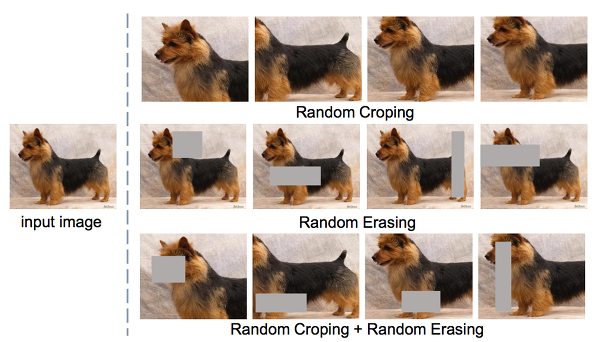
\includegraphics[width=0.6\textwidth]{img/data_augmentation.png}
        \caption{Verschiedene Methoden und Kombinationen zur Datenaugementation.}
        \label{fig:data_augmentation}
    \end{figure}
    
    Eine weitere Technik ist das Horizontale Spiegeln (Horizontal Flipping), bei dem die Bilder horizontal gespiegelt werden. Dadurch werden die Daten umgekehrt und das Modell lernt, Objekte aus verschiedenen Blickwinkeln zu erkennen. 
    Diese Technik ist besonders nützlich, wenn die Orientierung der Objekte in den Bildern nicht von Bedeutung ist.    
    Das Hinzufügen von Rauschen (Noise Addition) ist eine weitere Methode der Datenaugmentierung, bei der Rauschen in die Daten eingefügt wird.
    Dies kann helfen, das Modell widerstandsfähiger gegenüber Störungen zu machen und es auf den Umgang mit realen Daten vorzubereiten.    
    Weitere Techniken umfassen das Skalieren, Drehen, Farbveränderungen und das Hinzufügen von Text oder Objekten zu den Bildern. 

    \begin{figure}[!h]
        \centering
        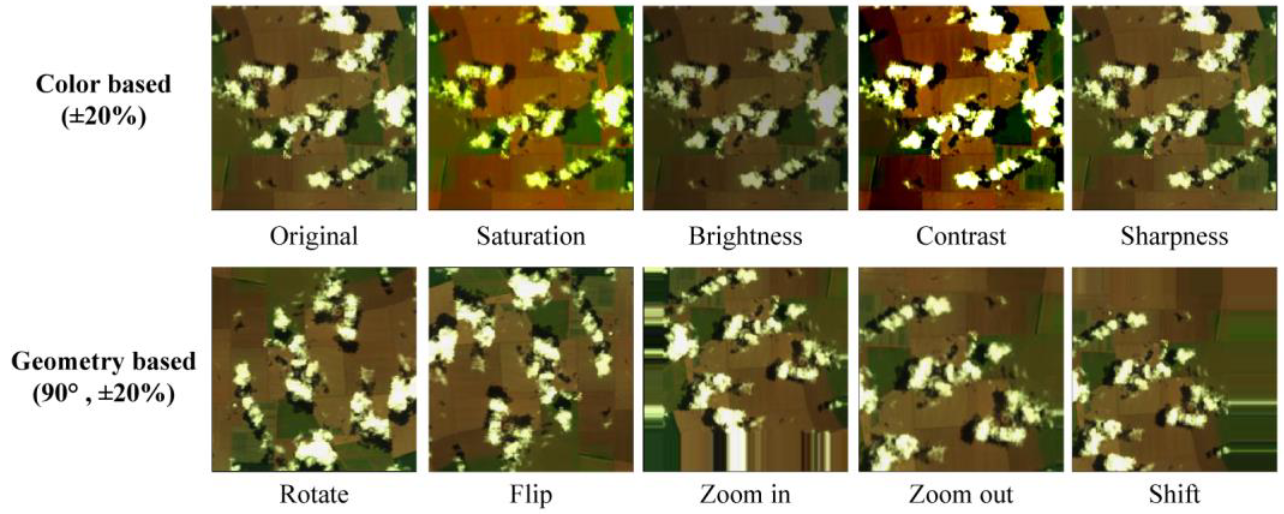
\includegraphics[width=0.6\textwidth]{img/data_augmentation_classics.png}
        \caption{Klassische Methoden und Kombinationen zur Datenaugementation.}
        \label{fig:data_augmentation_classics}
    \end{figure}
    
    Diese Methoden ermöglichen es, den Trainingsdatensatz zu diversifizieren und sicherzustellen, dass das Modell auf verschiedene Situationen und Variationen vorbereitet ist.    
    Insgesamt spielt die Datenaugmentierung eine bedeutende Rolle in der Datenverarbeitung, da sie die Qualität und Vielfalt der Trainingsdaten verbessert. 
    Durch die Anwendung verschiedener Transformationen auf die Daten kann das Modell robustere und leistungsfähigere Modelle erstellen. 
    Es ist wichtig, die richtigen Techniken der Datenaugmentierung entsprechend der Domäne und des Anwendungsfalls auszuwählen, um die Leistung des Modells zu verbessern.
    \footfullcite{shorten2019data,}

\section{Fazit}

Die richtige Vorverarbeitung der Daten ist entscheidend für den Erfolg von Modellen und Analysen. 
Durch Datenbereinigung, Datennormalisierung und Datenaugmentierung kann die Qualität und Aussagekraft der Daten verbessert werden, was zu besseren Ergebnissen führt. 
Die Datenbereinigung ermöglicht es, fehlerhafte oder unvollständige Daten zu entfernen oder zu korrigieren, um eine solide Grundlage für präzise und verlässliche Analysen und Modelle zu schaffen.

Obwohl in diesem Projekt der verwendete Datensatz bereits vorbereitet ist, ist es dennoch wichtig, zu prüfen, ob solch einer den Anforderungen des spezifischen Problems gerecht wird.
Dies könnte die Überlegung beinhalten, ob ein vorgefertigter Datensatz verwendet werden kann oder ob Anpassungen erforderlich sind, um sicherzustellen, dass die Daten die relevanten Informationen für die Analysen enthalten.
    